% master.tex : master-fil for projektet
% ------------------------------------------------------------------------------
% Dette er hovedfilen for projektet, hvori indhold fra alle input-filer (tekst,
% billeder, litteraturdatabaser, osv.) samles

% Dokumenttypen 'book' er valgt pga. dens mange fleksible indstillinger
% Se https://tex.stackexchange.com/a/36989/118167
\documentclass[11pt,a4paper,oneside,openright,danish]{book}

% Variabler, som bruges til automatisk at indsætte titel, forfattere, osv. på
% forsiden og titelbladet.
\def \projecttitle       {Optimering af gaslager}
\def \projectsubtitle    {Diskret optimering}
\def \projecttheme       {Optimering af gaslager}
\def \projectdegree      {Matematik-Økonomi}  % eller Matematik-Økonomi/Teknologi
\def \projectperiod      {Efterårssemesteret 2020}
\def \projectnumber      {P1}
\def \projectgroup       {B350}
\def \projectauthors     {
  Beate Marcussen\\
  Marcus Søndergaard Aaskoven\\
  Mathias Graversen\\
  Mattias Adam Arvidsson\\
  Vennan Vithiyatharan
  % ...
}
\def \projectsupervisors {
  Janus Valberg-Madsen\\
  % ...
}

% Preamblet indeholder alle de indstillinger og makroer, som skal indsættes for
% hovedindholdet, og i denne skabelon samles det i filen aaumath.sty, som
% definerer en pakke, der kan indlæses med \usepackage.
\usepackage{aaumath}
\usepackage{graphicx}
% Dokumentets indhold indsættes mellem \begin- og \end-makroerne for
% 'document'-blokken
\usepackage{amsthm}
\theoremstyle{definition}
\newtheorem{definition}
{Definition}[section]
\usepackage{mdframed}

\begin{document}

% Dokumentets 'front matter' tælles ikke med ifm. antal sider og nummereres med
% romerske tal. Herunder hører f.eks. forsiden, titelbladet, forordet og
% indholdsfortegnelsen.
\frontmatter
\include{incl/misc/frontpage}
\shipout\null
% incl/misc/titlepage.tex : rapportens titelblad
% ------------------------------------------------------------------------------
% Titelbladet genereres af makroen \aautitlepage, som er defineret i
% /incl/pre/ext/aautitlepage.sty


\pdfbookmark[0]{Titelblad}{titelblad}
\aautitlepage{
  \projectinfo{
    \projecttitle
  }{
    \projecttheme
  }{
    \projectperiod
  }{
    Gruppe \projectgroup
  }{
    \parbox[t]{\textwidth}{\projectauthors}
  }{
    \parbox[t]{\textwidth}{\projectsupervisors}
  }{
    \today
  }
}{
  \textbf{AAU First Year}\\
  Strandvejen 12-14\\
  DK-9000 Aalborg\\
  \href{http://math.aau.dk}{http://math.aau.dk}
}{
  % incl/misc/abstract.tex : projektets abstract
% ------------------------------------------------------------------------------
% Et abstract er et kort resume af rapporten, som vises på titelbladet
This study investigates how algorithms and graph teory can help optimze the profit of a gas storage in a given period of time by buying and selling gas units.
Initialy, relevant theory of graph theory and algorithms will be explained. The study found Dijkstra's algorithm very useful for solving the problem. By multiplaying by minus one and adding, so that no edges are negative, one can use an implementation of Dijkstra's algorithm in Python to find the longest path through a graph, by finding the shortest path through the inverted, positive graph. This path will be the path that yields the greatest profit. Furtermore the most profitable paths can be shown in graphs illustrating the best trading strategy. The greatest profit in the basic problem is 252.72 euros and the greatest profit in our extended problem is 188.27 euros. 
The extensions is seen to reduce the profit considerably, and  especially the fluctuating limits for inventory and sales per month are to blame for the low profit, as they affect profits over several months and not only in the last month, which the penalty factor does. 

}

\tableofcontents

% Dokumentets 'main matter' (hovedindhold) er der, hvor det meste indhold skal
% sættes ind. Sider og overskrifter er nummererede med arabiske tal.
\mainmatter

\chapter{Forord}
Følgende projekt er udarbejdet af gruppe B350 bestående af fire stud.scient.oeconer på 1. semester på Aalborg Universitet. Projektet er skrevet i efteråret 2020 og beskæftiger sig med diskret matematik herunder optimering af et gaslager. Diskret matematik indgår i studiets læreplan og er derfor et relevant emne til projektskrivning. Projektet er skrevet i \LaTeX \ og delt med Git via GitAhead. Til at løse vores problem har vi desuden opstillet algoritmer i Python 3.
Vi vil som gruppe rette en stor tak til vores vejleder Janus Valberg-Madsen for godt samarbejde gennem projektforløbet samt gode råd og rettelser.
\chapter{Indledning}
\section{Problemanalyse}
Klimakrisen har efterhånden været en del af den offentlige og politiske debat i mange år. For virksomheder kan det være svært at balancere mellem at være økonomisk effektiv og samtidig klimavenlig. Klimavenlige alternativer er nemlig ikke altid den mest profitable løsning. Derfor vurderes det mest klimavenlige alternativ ikke altid til at være specielt holdbart for virksomheder, men kan der findes et kompromis? 
\\

Hvis vi kigger på naturgas, indeholder det store mængder af metan, hvilket betyder en stor mængde af brint og knap så meget CO2 udslip. (https://www.experimentarium.dk/klima/naturgas/) Der udledes 40$\%$ mindre $CO_{2}$ sammenlignet med kul ved den samme mængde energi. Selvom naturgas er et fossilt brændstof, er det altså mere miljøvenligt end kul og olie, men for at få virksomheder til at benytte sig af denne form for energ, er det vigtigt at gøre det profitabelt for dem. Dette kan gøres ved at optimere deres processer.
Procesoptimering kan gøres på et utal af måder blandt andet ved at implementere en algoritme, der kan udregne, hvornår det er bedst at købe og sælge gassen, og hvor meget der skal købes eller sælges ad gangen. 
\\

I dette projekt vil vi arbejde med en sådan algoritme og bruge den til at optimere et gaslager, som vi vil leje for et år. Vi skal i denne periode forsøge at maksimere resultatet ved at købe og sælge gasenheder til forskellige tider med forudbestemte priser. Vi tager udgangspunkt i basisproblemet, men sørger for at algoritmen er optimeret således, at den er generel nok til at løse eventuelle udvidelser uden store ændringer.

\subsection{Problemformulering}
Dette leder os frem til følgende problemformulering:
\textit{Hvordan kan vi optimere profitten for et gaslager ved brug af grafteori og algoritmer, og kan vi generalisere løsningen udvide problemet?}

\section{Introduktion}
I denne rapport ønsker vi at optimere et gaslager ved at få det størst mulige resultat for det år vi vil leje det. Med problemet blev der også givet visse begrænsninger for gaslageret, herunder en nedre og en øvre grænse for, hvor meget gas lageret kan indeholde, samt en nedre og en øvre grænse for hvor meget gas der må købes og sælges hver måned. Der er dermed tale om et optimeringsproblem. 

Problemet kan beskrives matematisk ved hjælp af grafteori. Derfor vil der i dette projekt blive redegjort for centrale aspekter inden for grafteori såsom graftyper, repræsentation af grafer, veje og delte grafer. Med denne teori vil vi være i stand til at opstille en graf for vores problem. Vi vil dermed kunne finde den vej der giver den største profit. 
Dette kan dog være en langsommelig proces, derfor ønsker vi at opstille en algoritme, der kan udføre dette arbejde. Derfor vil vi også beskrive centrale elementer indenfor algoritmer. Vi vil først komme ind på nogle forskellige algoritmetyper. Herefter vil vi gennemgå Dijkstras algoritme, som bruges til at finde den korteste vej i en graf. Til sidst vil vi komme ind på kompleksitet, som giver et indblik i effektiviteten af algoritmer.





\chapter{Algoritmer} \label{kap.algo}
Når man står med et problem inden for diskret matematik, er det første, man skal gøre at finde en model, der kan sætte problemet i matematisk kontekst. Denne model skal bestå af diskrete strukturer såsom funktioner, sekvenser eller grafer, som vi omtalte i tidligere afsnit. Når man har opstillet en passende model til at løse problemet, skal man nu finde en metode, som kan løse det med denne model. Denne model skal helst tilpases så den kan løse det generelle problem. Det vil sige alle probemer af den type og form. Metode skal bestå af en række steps som slutteligt vil give resultatet. Disse steps kaldes en algoritme. 
\begin{defn}
[Algoritmer] En algoritme er en begrænset mængde af præcist definerede instruktioner, der viser hvordan et problem løses, eller hvordan en beregning udføres. 

\end{defn}
Der findes mange typer algoritmer, som løser mange forskellige problemer. Der er dog nogle kendetegn, som skal gøre sig gældende for alle algoritmer. Der skal være et input, og for hver inputværdi er der en outputværdi. Algoritmens steps skal være præcist defineret, så der ikke kan herske tvivl om, hvad der skal gøres i hvert step. En algoritme skal producere den korrekte outputværdi til hvert input. En algoritme er begrænset. Den kan have mange steps, men altså ikke ubegrænset, hvilket vil sige at den vil stoppe på et tidspunkt. En algoritme skal være effektiv, så man præcist og indenfor et begrænset tidsrum kan løse stepsene, og sidst men ikke mindst skal en algortime være generel, så den kan løse alle problemer af den type og form.

Selvom algoritmer alle har dette til fælles, er forskelligheden blandt dem stadig stor. Vi vil i det følgende se på forskellige typer af algoritmer.

\section{Dijkstras algoritme}
I \ref{defn:min.vej} definerede vi distancen af den korteste vej i en vægtet graf. For at finde den korteste vej vil vi anvende \emph{Dijkstras algoritme}. Dijkstras algoritme kan bruges til at finde den korteste vej i en simpel, vægtet graf, hvori vægtene for alle kanter i grafen skal være ikke-negative. Algoritmen fungerer således, at den finder den korteste vej fra en startknude, $v_{1}$, til en endeknude, $v_{m}$, ved først at finde naboknuderne til $v_{1}$ og undersøge hvilken af disse, der har den mindste distanceværdi og altså er tættest på startknuden. Derefter tager den udgangspunkt i den naboknude, hvortil distanceværdien er mindst og fortsætter ad dennes vej, så længe denne vej har en mindre distanceværdi end en alternativ vej. Fremgangsmåden vil her illustreres ved hjælp af et eksempel, som tager udgangspunkt i \ref{kap:grafteori}.

\begin{exmp} \label{exmp.dijkstae}
Betragt figur \ref{fig.dijkstraexmp}
\begin{figure}[H]
\centering
	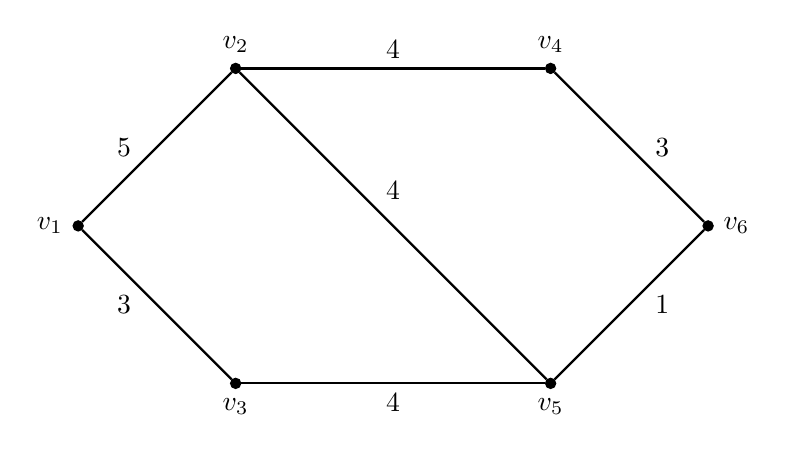
\begin{tikzpicture}

      \tikzset{enclosed/.style={draw, circle, inner sep=0pt, minimum size=.13cm, fill=black}}
%% Vertices
      	\node[enclosed, label={left: $v_1$}] (v1) at (0,2) {};
      	\node[enclosed, label={above: $v_2$}] (v2) at (2,4) {};
    	\node[enclosed, label={below: $v_3$}] (v3) at (2,0) {};
  	    \node[enclosed, label={above: $v_4$}] (v4) at (6,4) {};
     	\node[enclosed, label={below: $v_5$}] (v5) at (6,0) {};
     	\node[enclosed, label={right: $v_6$}] (v6) at (8,2) {};
%Edges
		\path [-, > = latex, thick] (v1) edge node[midway, left=2mm] {$ 5 $} (v2);
		\path [-, > = latex, thick] (v1) edge node[midway, left=2mm] {$ 3 $} (v3);
		\path [-, > = latex, thick] (v2) edge node[midway, above] {$ 4 $} (v4);
		\path [-, > = latex, thick] (v2) edge node[midway, above=2mm] {$ 4 $} (v5);
		\path [-, > = latex, thick] (v3) edge node[midway, below] {$ 4 $} (v5);
		\path [-, > = latex, thick] (v4) edge node[midway, right=2mm] {$ 3 $} (v6);
		\path [-, > = latex, thick] (v5) edge node[midway, right=2mm] {$ 1 $} (v6);

	\end{tikzpicture}
	\caption{Simpel, vægtet graf.}
	\label{fig.dijkstraexmp}
\end{figure}
I figur \ref{fig.dijkstraexmp} vil vi finde den korteste vej fra $v_{1}$ til $v_{6}$. Dijkstras algoritme vil gøre dette ved at finde den korteste vej fra startknuden, $v_{1}$, til hver knude, indtil den når endeknuden, $v_{6}$. Først vil den se, at startknuden har naboknuderne $v_{2}$ og $v_{3}$. Der er altså to veje fra startknuden, $P=(v_{1},v_{2})$ med distancen 5 og $P=(v_{1},v_{3})$ med distancen 3. Dermed er $v_{3}$ den knude, der er tættest på startknuden. Herefter er der igen to veje, $P=(v_{1},v_{2})$ med distancen 5 og $P=(v_{1},v_{3},v_{5})$ med distancen 7. Den første af disse vælges, da denne har den mindste distance, og $v_{2}$ er dermed knuden, som er næsttættest på startknuden. Nu er der tre forskellige veje, $P=(v_{1},v_{2}, v_{4})$ med distancen 9, $P=(v_{1},v_{2}, v_{5})$ med distancen 9 og $P=(v_{1},v_{3}, v_{5})$ med distancen 7. Den tredje vælges, og det er nu noteret, at den korteste vej fra $v_{1}$ til $v_{5}$ har distancen 7. Der er nu igen kun to mulige veje at vælge imellem, $P=(v_{1},v_{2}, v_{4})$ med distancen 9 og $P=(v_{1},v_{3}, v_{5}, v_{6})$ med distancen 8. $P=(v_{1},v_{2}, v_{5})$ er ikke længere en mulig vej, da vi allerede har fundet den korteste vej fra $v_{1}$ til $v_{5}$. Den anden vej har den mindste distance, og derfor vælger vi denne, og vi ved nu, at den korteste vej fra $v_{1}$ til $v_{6}$ er $P=(v_{1},v_{3}, v_{5}, v_{6})$ og har distancen 8.
\end{exmp}
Ovenstående eksempel er simpelt og kan hurtigt løses ved fx brute force metoden, men i større og mere komplicerede grafer er Dijkstras algoritme meget mere effektiv. For at skabe yderligere overblik over hvordan Dijkstras algoritme fungerer, vil vi her gå i dybden med dennes mere teoretiske del.
\begin{algorithm}[H]
\caption{Dijkstras algoritme}
\begin{algorithmic}[1]

\Procedure{dijkstra($G$: vægtet, forbundet, simpel graf med kun ikke-negative vægte)}{}
    \State \{$G$ {har knuderne $a = v_{1}, v_{2}, \dotsc, v_{m} = z$ og vægtene til kanterne $w(v_{i}, v_{j})$, hvor $w(v_{i}, v_{j}) = \infty$ hvis {$(v_{i}, v_{j})$} ikke er en kant i G\}}
	\For {$i := 2$ \textbf{to} $n$}
		\State $L(v_{i}) := \infty$
	\EndFor
	\State $L(a) := 0$	
	\State $S := \emptyset$
	\State {\{distancen til hver knude initialiseres, så $a = 0$, og distancen til alle andre knuder er $\infty$, derudover er $S$ defineret som en tom mængde\}}
    \While{$z \notin S$}
        \State {$u :=$ en knude som ikke er i $S$ med $L(u)$ som minimum}
        \State $S := S \cup \{u\}$
        \For {alle $v \notin S$}
        	\If {$L(u) + w(u,v) < L(v)$} {$L(v) := L(u) + w(u,v)$}
        	\State \{dette tilføjer knuder til $S$ med minimal 			distance og opdaterer distancerne til
        	\State knuderne, som ikke er i $S$\}
        	\EndIf
    	\EndFor
    \EndWhile
    \State {\textbf{return} $L(z)$ \{$L(z)$ er distancen af den korteste vej fra $a$ til $z$\}} 
\EndProcedure

\end{algorithmic}
\label{alg:dijkstra}
\end{algorithm}
Det første, der sker, er, at startknuden noteres som $0$, altså $v_{1} = 0$, og resten af knuderne noteres som $\infty$. Her betegnes den korteste vej som $\alpha_{k}(v_1,v_m)$, fra definition \ref{defn:min.vej}, hvor $k$ er antallet af \emph{iterationer} gennemført i algoritmen. Antallet af iterationer er det antal gange en løkke gennemkøres, altså hver gang vejen opdateres.  $\alpha_{0}(v_1,v_1)$ betyder altså, at vi har nul iterationer og dermed kun kender startknuden med distancen 0. Derudover oprettes en mængde $S$, for hvilken det gælder, at $S = \emptyset$ når $k = 0$. Ved første iteration undersøges startknudens naboknuder, og man bestemmer, som i eksemplet ovenfor, hvilken distance er mindst. Dermed er startknudens nærmeste knude fundet, og denne tilføjes nu til mængden $S$. For hver iteration tilføjes et nyt element til mængden, og denne proces fortsætter, til algoritmen har fundet den korteste vej fra startknuden til endeknuden. Mængden, $S$, indeholder til sidst distancerne for den korteste vej fra startknuden til alle knuder i grafen. 



\input{incl/main/algoritmer/viterbi}
\subsection{Grådige algoritmer}
Når man arbejder med optimeringsproblemer, som omhandler minimering eller maksimering, som fx kunne være at finde den længste eller korteste vej i en graf, kan man ofte bruge \emph{grådige algoritmer}.
En grådig algoritme vælger altid det \emph{lokalt optimale} valg og antager, at dette medfører en \emph{global optimal} løsning, altså den bedst mulige løsning. Det lokalt optimale valg findes ved at vælge den umiddelbart bedste løsning for hvert muligt trin.
I mange tilfælde vil dette lede til global optimering, men der kan også forekomme situationer, hvor algoritmen vil finde en suboptimal løsning. Ligegyldigt om algoritmen finder en optimal eller suboptimal løsning, kalder vi den en grådig algoritme. 
   
\autoref{fig:greedy.eks} er et eksempel på en grådig algoritme, som har forsøgt at finde den længst mulige simple vej i en graf.

\begin{figure}[H]
\centering
	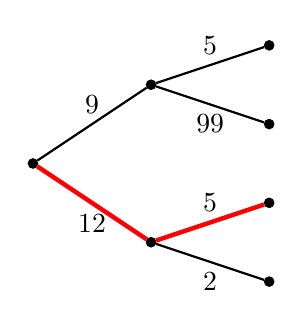
\begin{tikzpicture}

      \tikzset{enclosed/.style={draw, circle, inner sep=0pt, minimum size=.12cm, fill=black}}
% Vertices
      	\node[enclosed] (v1) at (0,2) {};
      	\node[enclosed] (v2) at (1.5,1) {};
    	\node[enclosed] (v3) at (1.5,3) {};
  	    \node[enclosed] (v4) at (3,0.5) {};
  	    \node[enclosed] (v5) at (3,1.5) {};
  	    \node[enclosed] (v6) at (3,3.5) {};
  	    \node[enclosed] (v7) at (3,2.5) {};    
%Edges
		\path[ultra thick] (v1) edge[red] node[midway, below, black] {$12$} (v2);
		\path[thick] (v1) edge node[midway, above] {$9$} (v3);
		\path[thick] (v2) edge[red, ultra thick] node[midway, above, black] {$5$} (v5);
		\path[thick] (v2) edge node[midway, below] {$2$} (v4);
		\path[thick] (v3) edge node[midway, above] {$5$} (v6);
		\path (v3) edge[thick] node[midway, below] {$99$} (v7);


	\end{tikzpicture}
	\caption{Længste vej, i simpel graf, ifølge grådig algoritme.}
	\label{fig:greedy.eks}
\end{figure}

Vi kan se, at algoritmen har valgt de lokalt optimale valg, men den har ikke fundet den globalt optimale løsning. Det er tydeligt at se, at denne algoritme ikke er pålidelig nok til at løse sådanne problemer, da den ikke konsekvent finder den globalt optimale løsning. Der findes dog nogle grådige algoritmer, som er optimeret, så de altid finder den globalt optimale løsning, så længe grafen overholder specifikke krav. Dette ser vi i \autoref{kap:dijkstras}.

    

\begin{exmp}
Det danske møntsystem har seks forskellige mønter med værdier på $0.5,\ 1,\ 2,\ 5,\ 10$ og $20$ kroner. Systemet er optimeret således, at man kan lave byttepenge vha. en grådig algoritme. Man kan altid finde den optimale løsning ved først at tage så mange som muligt af de mest værdifulde mønter, og derefter tager man så mange som muligt af de næstmest værdifulde mønter. Man fortsætter denne proces, indtil man har den ønskede mængde byttepenge.
\begin{algorithm} [H] 
\caption{Grådig algoritme til byttepenge}
\label{alg:byt}
\begin{algorithmic}[1]

\Procedure{Byttepenge($c_1,c_2,\dotsc,c_r$: værdien af mønter, hvor $c_1>c_2>\dotsb >c_r;n:$ et positivt heltal)}{}
\EndProcedure
\For{$i:=1$ \textbf{to} $r$}
    \State $d_i:=0$ ($d_i$ tæller mængden af mønter med værdi $c_i$)
    \While{$n \geq c_i$}
    	\State $d_i := d_i+1$ (Mængden af mønter med værdi $c_i$ øges med en.)
    	\State $n := n-c_i$
\EndWhile
\EndFor
\State ($d_i$ er mængden af mønter med værdi $c_i$ for $i=1,2,\dotsc,r$)
\end{algorithmic}
\end{algorithm}
Denne algoritme vil altid vælge den globalt optimale løsning i dette specifikke problem. Der kan dog være problemer, hvis mønternes værdi ændrer sig. 
Vi forestiller os nu, at vi har et møntsystem udelukkende med tre mønter af værdi $25$, $10$ og $1$. Der opstilles her et problem, hvor vi vil have $30$ kroner i byttepenge. \autoref{alg:byt} vil nu få en løsning, som bruger én mønt af værdi $25$ og fem mønter af værdi $1$. Dette er en suboptimal løsning, da man kunne have brugt tre mønter af værdi $10$.
Dette viser, at grådige algoritmer ikke altid finder den optimale løsning.
\end{exmp}


\section{Kompleksitet}
%side 250 ish
%table 1 side 247 i pdf.

Der findes to former for kompleksitet, men vi vælger at fokusere på tidskompleksitet. Den anden form for kompleksitet er pladskompleksitet. 
Der er tre former for tilfælde: bedste, værste og gennemsnitlige. 
I bedste tilfælde ser man på det laveste antal trin for en inputstørrelse, $n$. I værste ser man på det højeste og i gennemsnittet, det gennemsnitlige. 
\emph{Bedste tilfælde} beskriver algoritmen under optimale forhold, i en lineær søgealgoritme vil dette altså være, at elementet der søges efter, er det første element i listen. 
Oftere ser man på enten \emph{værste tilfælde} eller \emph{gennemsnitlige tilfælde}. 
Det gennemsnitlige tilfælde vil give et rigtigt godt overblik over hvor god algoritmen er, dog er det meget svært at bestemme hvad et gennemsnitligt input er, da det er svært at bestemme nogle parametre at vælge ud fra. 
Det værste tilfælde giver et godt overblik over hvor lang tid det kan tage. Ved man at algoritmen er lineær i værste tilfælde, vil man kunne løse den i rimelig tid for alle størrelser $n$.
De forskellige resultater i vores analyse af algoritmerne, kan deles op i kategorier, de mest gængse er: $\log n$, $\sqrt{n}$, $n$, $n^x$, $x^n$ og $n!$, men det kan også være en kombination af disse, som $n!n$, $n\log n$ eller lignende.
For at beskrive disse algoritmer i fx værste tilfælde, vil man bruge operatorerne \emph{store-O}, \emph{store-Omega} og \emph{Theta}. Man vil her fokusere på \emph{asymptotiske $n$-værdier}, altså ved rigtigt store værdier for $n$, da man i nogle tilfælde vil have en algoritme der er langsommere end den øvre bindende funktion ved små $n$, men ved større, som fx over 10.000, er hurtigere.

\subsection{store-$O$}
\begin{defn}
$f(n) = O(g(x))$ hvis og kun hvis $\exists$ positive konstanter $C$ og $n_o$ så at $f(n) \leq C g(n) \forall n \geq n_o$
\end{defn}

Store-$O$ bliver brugt til at binde funktionen opadtil, begrænse den oppe fra. Man kan med garanti sige, at algoritmen tager store-$O$ tid eller mindre. 
\begin{exmp}
\begin{align*}
f(n)=& 13n+3 \\
13n+3 \leq& 20n \forall \ n \geq 1 \\
f(n) =& O(n)
\end{align*}
\end{exmp}
Man vil også kunne sige, at $f(n)$ er mindre end $n!$ eller en anden vilkårlig højere funktion $g(n)$, men da man altid vil vælge den mest begrænsende funktion, vil $n$ være det mest præcise. 

\subsection{Store-$\Omega$}
\begin{defn}
$f(n) = \Omega(g(n))$ hvis og kun hvis $\exists$ positive konstanter $C$ og $n_o$ så at $f(n) \geq C g(n) \forall n \geq n_o$
\end{defn}
Store-Omega bruges, omvendt store-$O$, til at binde funktionen nedadtil, altså finde den nedre grænse for algoritmen, den vil mindst tage store-Omega tid i det givne tilfælde.
\begin{exmp}
\begin{align*}
f(n)=& 13n+3 \\
13n+3 \geq& n \forall \ n \geq 1 \\
f(n) =& \Omega(n)
\end{align*}
\end{exmp}

På samme måde som ved store-$O$-notationen, vil man her kunne vælge en vilkårlig mindre funktion, $logn$, $1$ med flere, men da man vil begrænse den så meget som muligt, vælger man den største funktion $g(n)$ hvor uligheden stadig er sand.
\subsection{Theta}
\begin{defn}
$f(n) = \Theta(g(x))$ hvis og kun hvis $\exists$ positive konstanter $C_1, C_2$ og $n_o$ så at $C_1g(n) \leq f(n) \leq C_2g(n) \forall n \geq n_o$
\end{defn}
Når man har fundet den øvre og den nedre grænse, store-O og store-Omega, kan man finde Theta, den tætte bundne funktion,
\begin{exmp}
\begin{align*}
f(n)=& 13n+3 \\
n \leq 13n+3 \leq& 10n \forall \ n \geq 1 \\
f(n) =& \Theta(n)
\end{align*}
\end{exmp}
P \\
NP \\
NP-Complete \\
NP-Hard. 

Store-O
O
Store-Omega

Theta
store-Theta

\section{Algoritmetyper}
Der findes mange typer algoritmer, som løser mange forskellige problemer. Vi vil i det følgende se på forskellige typer af algoritmer.
\subsection{Søgealgoritmer}
\emph{Søgealgoritmer} bruges til at løse problemer, hvor man vil finde et element, $x$, i en liste $(a_{1}, a_{2}, \dotsc, a_{n})$, eller konkludere, at $x$ ikke er i listen. Her vil løsningen være $i$, hvis $x=a_{i}$. Det er altså indekset, der er løsningen. Der findes forskellige søgealgoritmer bl.a. \emph{den lineære søgning} og \emph{den binære søgning}. Ved den lineære søgning starter man med $a_1$ og ser, om $x=a_{1}$. Hvis dette er tilfældet, er $a_{1}$'s indeks svaret, men hvis $x \neq a_{1}$, fortsætter man til $a_{2}$ og så $a_{3}$. Sådan fortsætter man, indtil man finder et element i listen, der er lig $x$, hvis et sådant element eksisterer. Hvis dette er tilfældet, returnerer algoritmen elementets indeks og ellers returnerer den 0. \autoref{alg:lineaer} illustrerer et eksempel på en lineær søgealgoritme:

\begin{algorithm}[H] 
\caption{Den lineære søgealgoritme}
\begin{algorithmic}[1]

\Procedure{lineær søgning($x$: heltal, $a_{1},a_{2},\dotsc,a_{n}$: Heltal i listen)}{}
    \State $i:=1$
    \While{$i \leq n$ \textbf{and} $x \neq a_{i}$}
        \State $i:=i+1$
    \EndWhile
    \If{$i \leq n$} 
    \State \textbf{return} $lokation:=i$
    \Else
    \State \textbf{return} $lokation:=0$
    \EndIf
  \label{roy's loop}
\EndProcedure

\end{algorithmic}
\label{alg:lineaer}
\end{algorithm}


Modsat den lineære søgning kan den binære søgning kun bruges, når en liste er \emph{ordnet}. Det vil sige, hvis listen fx er voksende, aftagende eller alfabetisk, altså $(a_{1}<a_{2}<\dotsb<a_{n})$. Den binære søgealgoritme finder nu midten af listen, $a_{m}$, hvor $m=\left \lfloor \frac{n+1}{2} \right \rfloor$. $\lfloor \ \rfloor$ er flooroperatoren, der runder ned til første heltal. Vi ser nu, hvilken side det, vi søger, er på. Hvis $a_{m}<x$, tager vi halvdelen af listen, der er større end $a_{m}$ dvs: $(a_{m+1}, a_{m+2},\dotsc,a_{n})$. Ellers tager vi halvdelen mindre end og lig $a_{m}$: $(a_{1}, a_{2},\dotsc,a_{m})$. Når vi har vurderet hvilken side af midten, den værdi, vi søger, er på, deles denne halvdel på midten, hvorefter man igen skal vurdere, hvilken side man skal arbejde videre med. Dette fortsættes, indtil tallet er fundet. Den binære søgealgoritme er illustreret i \autoref{alg:binaer}.

\begin{algorithm}[H]
\caption{Den binære søgealgoritme}
\begin{algorithmic}[1]

\Procedure{binær søgning($x$: heltal, $a_{1},a_{2},\dotsc,a_{n}$: Voksende heltal i listen)}{}
    \State $i:=1$, \{$i$ er venstre endepunkt i søgeintervallet\}
    \State $j:=n$, \{$j$ er højre endepunkt i søgeintervallet\}
    \While{$i<j$}
        \State $m=\lfloor (i+j)/2 \rfloor$
    		\If{$x>a_{m}$}
    		\State $i:=m+1$
    		\Else
    		\State $j:=m$
    		\EndIf    
    \EndWhile
    \If {$x=a_{i}$}
    	\State \textbf{return} $lokation:=i$
    \Else
    	\State \textbf{return} $lokation:=0$
    \EndIf
  \label{roy's loop}
\EndProcedure

\end{algorithmic}
\label{alg:binaer}
\end{algorithm}

\subsection{Sorteringsalgoritmer} \label{kap:sortering}
Når vi arbejder med \emph{sorteringsalgoritmer}, er det, fordi vi ønsker at sortere en liste, således at den inddeles i fx voksende rækkefølge eller alfabetisk orden. Ligesom ved søgealgoritmerne er der flere forskellige sorteringsalgoritmer. Eksempler på disse er \emph{bubblesortering} og \emph{indskudssortering}. Bubblesortering er en af de simpleste sorteringsalgoritmer, men den er ikke så effektiv. Den sammenligner tilstødende værdier i en liste og bytter om på dem, hvis rækkefølgen ikke er korrekt. Vi vil komme ind på algoritmers effektivitet i \autoref{kap:kompleksitet}.

\begin{algorithm}[H]
\caption{Bubblesorteringsalgoritmen}
\begin{algorithmic}[1]

\Procedure{bubblesortering($a_{1},a_{2},\dotsc,a_{n}$: Reelle tal hvor $n \geq 2$)}{}
\EndProcedure
\For {$i:=1$ \textbf{to} $n-1$}
    	\For {$j:=1$ \textbf{to} $n-i$}
    		\If {$a_{j}>a_{j+1}$}
    			\State Ombyt $a_{j}$ og $a_{j+1}$ 	
\EndIf
\EndFor
\EndFor
\State $a_{1},a_{2},\dotsc,a_{n}$ er i voksende rækkefølge. 

\end{algorithmic}
\end{algorithm}

\begin{exmp}
Vi ser på en liste, $(3,4,2,5,1)$, som vi vil arrangere således, at den er i rækkefølge med stigende værdi. Algoritmen gentages fire gange, da listen har længden $n=5$, og algoritmen skal køre $n-1$ gange. 
\begin{align*}
	\text{Første gentagelse:} \qquad \qquad \qquad \quad \text{Anden 			gentagelse:} \qquad \qquad \qquad \quad \text{Tredje gentagelse:} 			\qquad \qquad \qquad \quad \\
	(\textbf{3,4},2,5,1) \rightarrow (\textbf{3,4},2,5,1) \qquad \qquad 		(\textbf{3,2},4,1,5) \rightarrow (\textbf{2,3},4,1,5) \qquad \qquad 		(\textbf{2,3},1,4,5) \rightarrow (\textbf{2,3},1,4,5) \qquad \qquad 		\\
	(3,\textbf{4,2},5,1) \rightarrow (3,\textbf{2,4},5,1) \qquad \qquad     	(2,\textbf{3,1},4,5) \rightarrow (2,\textbf{1,3},4,5) \qquad \qquad   	(2,\textbf{3,1},4,5) \rightarrow (2,\textbf{1,3},4,5) \qquad \qquad 		\\
	(3,2,\textbf{4,5},1) \rightarrow (3,2,\textbf{4,5},1) \qquad \qquad 		(2,1,\textbf{3,4},5) \rightarrow (2,1,\textbf{3,4},5) \qquad \qquad  	\qquad \qquad \qquad \qquad \qquad \qquad \qquad \quad \ \ \\
	(3,2,4,\textbf{5,1}) \rightarrow (3,2,4,\textbf{1,5}) \qquad \qquad 		\qquad \qquad \qquad \qquad \qquad \qquad \qquad \quad \ \  \qquad 			\qquad \qquad \qquad \qquad \qquad \qquad \quad \ \
\end{align*}

\begin{flushleft}
Fjerde gentagelse:
\\
$(\textbf{2,1},3,4,5) \rightarrow (\textbf{1,2},3,4,5)$
\end{flushleft}

Efter første gentagelse har algoitmen placeres det største tal bagerst i listen, efter anden gentagelse har algoritmen placeret det næst største tal på næst sidste plads i listen. Således fortsætter algoritmen indtil listen er i korrekt rækkefølge.

\end{exmp}

Indskudssortering er på samme måde som bubblesortering simpel og til tider ineffektiv. For denne algoritme gælder det, at man starter med den anden værdi i listen, som sammenlignes med den første værdi. Disse to sorteres nu efter størrelse. Den tredje værdi i listen sammenlignes derefter med den første. Hvis den er større, sammenlignes den med den anden værdi i listen, og på den måde sorteres hele rækken, så de til sidst står i rækkefølge.

\begin{algorithm}[H]
\caption{Indskudssorteringsalgoritmen}
\begin{algorithmic}[1]

\Procedure{indskudssortering($a_{1},a_{2},\dotsc,a_{n}$: Reelle tal hvor $n \geq 2$)}{}
\EndProcedure
\For {$j:=2$ \textbf{to} $n$}
	\State $i:=1$
    	\While {$a_{j}>a_{i}$}
    		\State $i:=i+1$
    	\EndWhile
    	\State $m:=a_{j}$
    	\For {$k:=0$ \textbf{to} $j-i-1$}
    		\State $a_{j-k}:=a_{j-k-1}$
    	\EndFor
    	\State $a_{i}:=m$
\EndFor
\State $a_{1},a_{2},\dotsc,a_{n}$ er i voksende rækkefølge. 

\end{algorithmic}
\end{algorithm}

\begin{exmp}
Vi ser igen på en liste, $(3,4,2,5,1)$, som vi gerne vil sortere i rækkefølge, således at de står med stigende værdi. Til at gøre dette, vil vi bruge indskudssorteringsalgoritmen. Illustrationen, som ses nedenfor, viser, at alle understregede tal står i korrekt rækkefølge. Tallet markeret med fed er det næste tal, som algoritmen skal placere i den korrekte liste.

\begin{figure}[H]
\label{fig:indskud}
	\begin{flushleft}
	$i=1: \ (\underline{3},\textbf{4},2,5,1) \rightarrow (\textbf{4}, \underline{3},2,5,1)\rightarrow (\underline{3,\textbf{4}},2,5,1)$ \\
	$i=2: \ (\underline{3,4},\textbf{2},5,1) \rightarrow (\underline{\textbf{2},3,4},5,1) $\\
	$i=3: \ (\underline{2,3,4},\textbf{5},1) \rightarrow (\textbf{5},\underline{2,3,4},1) \rightarrow (\underline{2}, \textbf{5},\underline{3,4},1) \rightarrow (\underline{2,3}, \textbf{5}, \underline{4},1) \rightarrow (\underline{2,3,4,\textbf{5}},1) $ \\
	$i=4: \ (\underline{2,3,4,5},\textbf{1}) \rightarrow (\underline{\textbf{1},2,3,4,5}) $\\
 	\end{flushleft}
\end{figure}

Vi kan se, at algoritmen starter med at sammenligne fire med tre. Den tjekker først om fire er mindre end tre. Da det er større og der ikke er flere tal i listen, placeres fire i slutningen af den korrekte liste. Den tjekker nu det tredje tal i listen og ser med det samme, at det er mindre end det første tal i den korrekte liste. Derfor placeres to på den første plads i den korrekte liste. Den sammenligner nu fem med alle tal i den korrekte liste, og placerer fem efter det største tal den er større end. Dette gør den med alle tallene i listen, og den har til sidst placeret alle tallene i listen i korrekt rækkefølge.


\end{exmp}
Skriver bare herinde så den ikke slettes.
\chapter{Grafteori}
Følgende kapitel er skrevet med afsæt i \citep{dmat}.

Grafer er diskrete strukturer bestående af et antal knuder, samt et antal kanter, der forbinder disse knuder. Eksisterer der en kant mellem to knuder, siger vi, at denne kant forbinder knuderne. Det kaldes også, at kanten er incident med knuderne. Hvis en kant kun er incident med én knude, er der tale om en løkke. Knuderne illustreres ofte som prikker, mens kanterne repræsenteres af streger eller pile, der forbinder disse prikker. Graferne varierer alt efter deres type og funktion. De mange forskellige egenskaber betyder, at problemer i næsten enhver tænkelig disciplin kan løses ved hjælp af grafmodeller. Vi vil eksempelvis i dette projekt benytte grafteori og princippet om den længste vej til at optimere et gaslager.

\section{Graftyper}
En graf er, som tidligere nævnt, en struktur med knuder og kanter. Den er givet ved definitionen:
\begin{defn}
[Simpel graf] 
En graf, $G=(V,E)$, består af $V$, en mængde af \emph{knuder}, hvor $V = \emptyset$, og en mængde af \emph{kanter}, $E \subseteq \{\{u,v\}|u,v \in V\}$.
\end{defn}
Det fremgår af definitionen, at en graf ikke kan have nul knuder, men en lignende afgrænsning i den anden ende eksisterer ikke. Der kan dermed være uendeligt mange knuder. På samme måde gælder det for kanter, at der kan være mellem nul og uendeligt. Hvis mindst et af disse tilfælde gør sig gældende, kaldes det en \emph{uendelig graf}. Ellers kaldes det en \emph{endelig graf}, og det er denne type, som vi beskæftiger os med i projektet.
Ydermere, ses det i definitionen, at hver kant forbinder én eller to knuder. For en simpel graf gælder det, at ingen kanter forbinder et punkt med sig selv. Der må altså ikke være løkker. 

\begin{figure}[H]
\centering
	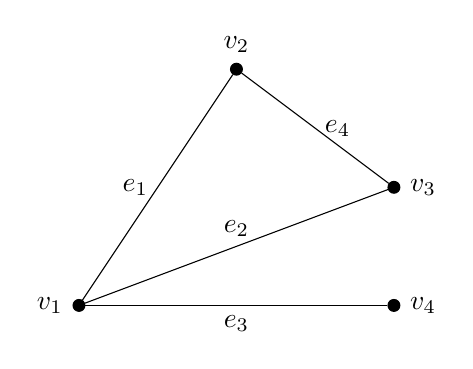
\begin{tikzpicture}

      \tikzset{enclosed/.style={draw, circle, inner sep=0pt, minimum size=.15cm, fill=black}}
%% Vertices
      	\node[enclosed, label={left: $v_1$}] (v1) at (0,0) {};
      	\node[enclosed, label={above: $v_2$}] (v2) at (2,3) {};
    	\node[enclosed, label={right: $v_3$}] (v3) at (4,1.5) {};
  	    \node[enclosed, label={right: $v_4$}] (v4) at (4,0) {};
%Edges
		\path (v1) edge node[midway, left] {$e_1$} (v2);
		\path (v1) edge node[midway, above] {$e_2$} (v3);
		\path (v1) edge node[midway, below] {$e_3$} (v4);
		\path (v2) edge node[midway, right] {$e_4$} (v3);

	\end{tikzpicture}
	\caption{En simpel graf}
	\label{fig.simpel}
\end{figure}



I kontrast til den simple graf finder vi multigrafen. For denne type graf skal der være flere kanter, der forbinder det samme knudepar. Der må stadig ikke optræde løkker.

\begin{figure}[H]
\centering
	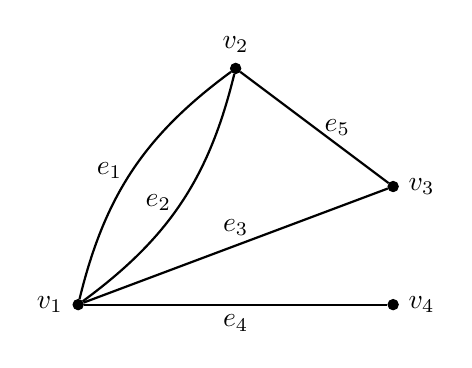
\begin{tikzpicture}

      \tikzset{enclosed/.style={draw, circle, inner sep=0pt, minimum size=.13cm, fill=black}}
%% Vertices
      	\node[enclosed, label={left: $v_1$}] (v1) at (0,0) {};
      	\node[enclosed, label={above: $v_2$}] (v2) at (2,3) {};
    	\node[enclosed, label={right: $v_3$}] (v3) at (4,1.5) {};
  	    \node[enclosed, label={right: $v_4$}] (v4) at (4,0) {};
%Edges
		\path[thick] (v1) edge [bend right=20] node[midway, left] {$e_2$} (v2);
		\path[thick] (v2) edge [bend right=20] node[midway, left] {$e_1$} (v1);
		\path[thick] (v1) edge node[midway, above] {$e_3$} (v3);
		\path[thick] (v1) edge node[midway, below] {$e_4$} (v4);
		\path[thick] (v2) edge node[midway, right] {$e_5$} (v3);

	\end{tikzpicture}
	\caption{En multigraf.}
	\label{fig.multi}
\end{figure}


En pseudograf er en graf, der \emph{kan} indeholde løkker, men generelt set er alle grafer pseudografer. Man vil dog kun bruge betegnelsen, pseudograf, hvis den indeholder en løkke, da det ellers vil være mere præcist at kalde den en simpel eller multigraf. Vi ser i eksemplet herunder, at der er to kanter, der forbinder $v_{1}$ og $v_{2}$, og der er en løkke ved $v_{4}$.

\begin{figure}[H]
\centering
	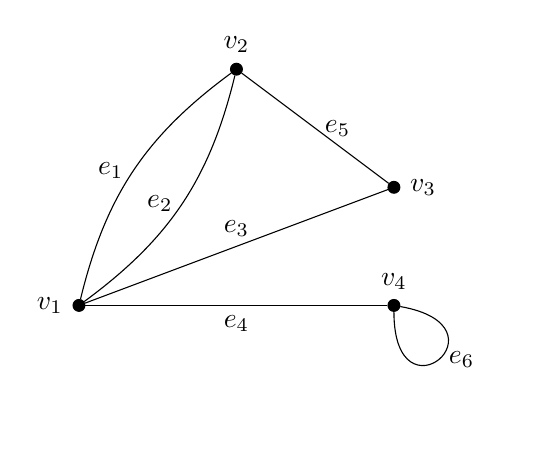
\begin{tikzpicture}[every loop/.style={}]
      \tikzset{enclosed/.style={draw, circle, inner sep=0pt, minimum size=.15cm, fill=black}}
%% Vertices
      	\node[enclosed, label={left: $v_1$}] (v1) at (0,0) {};
      	\node[enclosed, label={above: $v_2$}] (v2) at (2,3) {};
    	\node[enclosed, label={right: $v_3$}] (v3) at (4,1.5) {};
  	    \node[enclosed, label={above: $v_4$}] (v4) at (4,0) {};
%Edges
		\path (v1) edge [bend right=20] node[midway, left] {$e_2$} (v2);
		\path (v2) edge [bend right=20] node[midway, left] {$e_1$} (v1);
		\path (v1) edge node[midway, above] {$e_3$} (v3);
		\path (v1) edge node[midway, below] {$e_4$} (v4);
		\path (v2) edge node[midway, right] {$e_5$} (v3);
		\path (v4) edge [out=270,in=350,looseness=35] node[right] {$e_6$} (v4);
	\end{tikzpicture}
	\caption{En pseudograf med en løkke.}
	\label{fig.pseudo}
\end{figure}



\subsection{Orienterede grafer og ikke-orienterede grafer}
En anden typisk grafopdeling er opdelingen i orienterede og ikke-orienterede grafer. De grafer, vi har kigget på indtil videre, er ikke-orienterede grafer. For en orienteret graf gælder det, at grafens kanter er retningsbestemte. Dette er ofte illustreret med pile. Den har dermed en startknude og en endeknude. Disse grafer er defineret ved:

\begin{defn}
[Orienteret graf] 

En orienteret graf, $G=(V,E)$, består af $V$, en m�ngde knuder, hvor $V \neq \emptyset$, og en mængde orienterede kanter, $E$. Hver orienterede kant forbinder et par knuder, $(u,v)$, hvor startknuden, $u$, er tilstødende til endeknuden, $v$. 


\input{fig/tikz/grafer/graftyper/orienteretgraf}

Der kan foruden disse to også være tale om blandede grafer, som er grafer med både orienterede og ikke-orienterede kanter. Orienterede grafer kan ligesom ikke-orienterede grafer indeholde løkker og flere ensrettede kanter, der forbinder det samme par knuder, men hvis dette ikke er tilfældet, kaldes det en orienteret simpel graf. En orienteret simpel graf må også indeholde to modsatrettede kanter mellem det samme knudepar. Dermed kan en kant gå fra $v$ til $u$, selvom en anden kant går fra $u$ til $v$. Hvis der derimod optræder løkker eller flere ensrettede kanter mellem et eller flere knudepar, kaldes det en orienteret multigraf.  

Egenskaberne for de forskellige grafer kan ses herunder:


\begin{center}
\begin{tabular}{ |p{4cm}|p{3cm}|p{3cm}|p{2cm}|  }
 \hline
 \multicolumn{4}{|c|}{Grafer} \\
 \hline
 Type & Kanter & Flere kanter per knudepar tilladt & Løkker tilladt\\
 \hline
 Simpel graf   & Ikke-orienterede    & Nej &   Nej\\
 Multigraf &   Ikke-orienterede & Ja   & Nej\\
 Pseudograf & Ikke-orienterede & Ja &  Ja\\
 Simpel orienteret graf    & Orienterede & Nej &  Nej\\
 Orienteret multigraf &  Orienterede  & Ja & Ja\\
 Blandet graf & Ikke-orienterede og orienterede  & Ja   & Ja\\
 \hline
\end{tabular}
\end{center}

Fordi kanterne i grafer med orienterede kanter er ordnede par, kan definitionen af knudens grader være antallet af kanter, der har denne knude som begyndelsesknude, eller antallet af kanter, der har denne knude som endeknude:
\begin{defn}
[Graden af en orienteret graf] 
I en graf med orienterede kanter er ind-graden, betegnet ved $deg^{-}(v)$, antallet af kanter med $v$ som deres endeknude. Ud-graden, betegnet ved $deg^{+}(v)$, er antallet af kanter med $v$ som deres startknude.
\end{defn}
Vi vil i projektet beskæftige os med orienterede grafer, da det er denne type, vi bruger til optimering af gaslageret. I vores tilfælde vil vi tildele vores orienterede kanter vægt, hvilket beskrives senere i projektet.


\section{Repræsentation af grafer}
Inden for grafteori er der forskellige måder at repræsentere en graf på. Normalvis repræsenterer man en graf med punkter og streger og/eller pile, men de kan også repræsenteres ved brug af lister og matricer. Disse metoder giver et mere praktisk overblik over grafer.

\subsection{Nabolister}
En måde at repræsentere en graf på er ved at lave en naboliste. Nabolister er tabeller, der giver en oversigt over hvilke knuder, der er forbundet med andre knuder. Dog vil man ikke kunne se, hvis der er parallelle kanter. En naboliste er bygget op således, at knuden, man vil beskrive, er i venstre side af tabellen, og naboknuderne er skrevet i højre side. \\

%\begin{figure}[h]
%  \centering
%  \begin{tikzpicture}
%    \node[point] at (1,2) ($v_{2}$) [label=above:\(A\)] {};
%    \node[point] at (3,2) ($v_{4}$) [label=above:\(B\)] {};
%    \node[point] at (4,1) ($v_{7}$) [label=right:\(C\)] {};
%    \node[point] at (2,0) ($v_{5}$) [label=below:\(D\)] {};
%    \node[point] at (3,0) ($v_{6}$) [label=below:\(E\)] {};
%    \node[point] at (1,1) ($v_{3}$) [label=left:\(F\)] {};
%    \node[point] at (0,2) ($v_{1}$) [label=below:\(G\)] {};
%
%    \footnotesize
%    \draw ($v_{2}$) -- ($v_{1}$);
%    \path ($v_{3}$) edge [bend left] ($v_{4}$);
%    \draw ($v_{2}$) -- ($v_{3}$);
%    \path ($v_{3}$) edge [bend right] ($v_{4}$);
%    \draw ($v_{4}$) -- ($v_{5}$);
%    \draw ($v_{4}$) -- ($v_{6}$);
%    \draw ($v_{4}$) -- ($v_{5}$);
%    \draw ($v_{7}$) -- ($v_{6}$);
%    \draw ($v_{7}$) to [out=315,in=45,looseness=50] ($v_{7}$);
%    \draw ($v_{6}$) -- ($v_{5}$);
%    \draw ($v_{5}$) -- ($v_{3}$);
%    \draw ($v_{3}$) -- ($v_{1}$);
%  \end{tikzpicture}
%  \caption{Ikke-orienteret pseudograf.}
%  \label{fig:ikke-orienteret-pseudo}
%\end{figure}

\begin{center}
	\begin{tabular}{ |p{4cm}||p{3cm}|}
	 	\hline
 		\multicolumn{2}{|c|}{Naboliste til figur \ref{fig:ikke-orienteret-pseudo}} \\
 		\hline
 		Knuder & Naboknuder\\
 		\hline
 		A & F,G \\
		B & C,D,E,F \\
		C & B,E,C \\
		D & B,E,F \\
		E & B,C,D \\
		F & A,B,D,G \\
		G & A,F \\
 	\hline
 	\label{tab:naboliste} 	
	\end{tabular}
	%\caption{Naboliste til figur \ref{fig:ikke-orienteret-pseudo}
\end{center}
Ud fra tabellen ses, at knuden B har naboknuderne C, D, E og F, men man kan ikke se, at der er en ekstra kant mellem B og F. Dog kan man se, at C har en løkke, da den er nabo til sig selv.

\begin{figure}[H]
  \centering
  \begin{tikzpicture}
    \node[point] at (1,2) (A) [label=above:\(A\)] {};
    \node[point] at (3,2) (B) [label=above:\(B\)] {};
    \node[point] at (4,1) (C) [label=right:\(C\)] {};
    \node[point] at (2,0) (D) [label=below:\(D\)] {};
    \node[point] at (3,0) (E) [label=below:\(E\)] {};
    \node[point] at (1,1) (F) [label=left:\(F\)] {};
    \node[point] at (0,2) (G) [label=below:\(G\)] {};

    \footnotesize
    \path [->] (A) edge [bend left] (G);
    \path [->] (A) edge [bend right] (G); 
    \path [->] (F) edge [bend left] (B);
    \draw [<-](A) -- (F);
    \path [<-](F) edge [bend right] (B);
    \draw [->](B) -- (D);
    \draw [<-](B) -- (E);
    \draw [<-](B) -- (C);
    \draw [->](C) -- (E);
    \draw [->](C) to [out=315,in=45,looseness=50] (C);
    \draw [<-](E) -- (D);
    \draw [->](D) -- (F);
    \draw [->](F) -- (G);
  \end{tikzpicture}
  \caption{Orienteret pseudograf.}
  \label{fig:orienteret-pseudo}
\end{figure}

%\begin{center}
%	\begin{tabular}{ |p{4cm}||p{3cm}|}
%	 	\hline
% 		\multicolumn{2}{|c|}{Naboliste til figur \ref{fig:orienteret-pseudo} \\
% 		\hline
% 		Knuder & Naboknuder\\
% 		\hline
% 		A & G \\
%		B & D,F \\
%		C & B,E,C \\
%		D & E,F \\
%		E & B \\
%		F & A,B,G \\
%		G &  \\
% 	\hline
% 	\label{tab:naboliste1}
%	\end{tabular}
%\end{center}

\ref{tab:naboliste1} viser en oversigt over den orienterede grafs (Figur \ref{fig:orienteret-pseudo}) naboknuder. Kigger man på B og F i tabellen, kan man se, at der er parallelle kanter, da kanterne er orienteret i hver deres retning. Kigger man på A og G, kan man ikke se, at der er parallelle kanter mellem A og G, da begge kanter er orienteret fra A til G.

\subsection{Nabomatricer}
En anden mulighed for at repræsentere en graf er ved brug af \emph{nabomatricer}. Nabomatricer er bedre, når grafen har mange kanter, da man her kan se hvor mange kanter et givent knudepar har.
En nabomatrix kan beskrives som en $N=m \times m$-matrix, hvor $m$ er afhængig af knudemængden $V=\{v_1, v_2, \dotsc, v_m\}$. Hvis man har en simpel graf, $G=(V,E)$, vil matricen være en 0-1-matrix, da en simpel graf kun kan have en kant mellem to knuder. Når der er en kant mellem to  vilkårlig knuder, $a_{ij}=(v_i,v_j)$,  vil den få notationen 1, hvis der derimod ikke er en kant, får den notationen 0.
Det kan også skrives som
\begin{equation}
	a_{ij} =	
	\begin{cases}
		1 \mbox{ hvis } (v_i,v_j) \\
		0 \mbox{ ellers }.
	\end{cases}
\end{equation}

\begin{figure}[H]
  \centering
  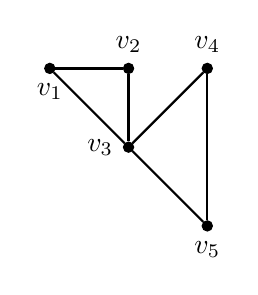
\begin{tikzpicture}
  \tikzset{enclosed/.style={draw, circle, inner sep=0pt, minimum size=.13cm, fill=black}}
  	\node[enclosed] at (0,2) (v1) [label=below:\(v_1\)] {};
    \node[enclosed] at (1,2) (v2) [label=above:\(v_2\)] {};
    \node[enclosed] at (1,1) (v3) [label=left:\(v_3\)] {};
    \node[enclosed] at (2,2) (v4) [label=above:\(v_4\)] {};
    \node[enclosed] at (2,0) (v5) [label=below:\(v_5\)] {};
    
	\path[thick] (v1) edge node {} (v2);
	\path[thick] (v1) edge node {} (v3);
	\path[thick] (v2) edge node {} (v3);
	\path[thick] (v4) edge node {} (v3);
	\path[thick] (v5) edge node {} (v3);   
	\path[thick] (v4) edge node {} (v5); 

  \end{tikzpicture}
  \caption{Ikke-orienteret, simpel graf til matrix.}
  \label{fig:stm}
\end{figure}

Nabomatricen nedenfor, viser en matrix over \autoref{fig:stm}.
\begin{equation}
	\begin{bmatrix}
		&v_1&v_2&v_3&v_4&v_5 \\
		v_1&0&1&1&0&0 \\
		v_2&1&0&1&0&0 \\
		v_3&1&1&0&1&1 \\
		v_4&0&0&1&0&1 \\
		v_5&0&0&1&1&0 \\
	\end{bmatrix}
\end{equation}

En matrix over en graf med flere parallelle kanter mellem to knuder vil se ud således. Matricen nedenfor viser en matrix over \autoref{fig:ikke-orienteret-pseudo}.

\begin{equation}
	\begin{bmatrix}
	&v_1&v_2&v_3&v_4&v_5&v_6&v_7& \\
	v_1&0&1&1&0&0&0&0 \\
	v_2&1&0&1&0&0&0&0 \\
	v_3&1&1&0&2&1&0&0 \\
	v_4&0&0&2&0&1&1&1 \\
	v_5&0&0&1&1&0&1&0 \\
	v_6&0&0&0&1&1&0&1 \\
	v_7&0&0&0&1&0&1&1 \\	
	\end{bmatrix}
\end{equation}

Det kan ses, at der er 2 kanter, der er incidente med knudeparret $v_3$ og $v_4$. Derudover kan det ses, at der er en løkke ved $v_7$.



\section{Veje}
Vi har indtil videre snakket om knuder, og hvordan de som knudersæt forbindes med kanter. I dette afsnit vil vi udvide det til at snakke om veje, som er sekvenser af disse kanter. Hvis der er tale om ikke-orienterede grafer, er veje defineret ved:
\begin{defn}
[Veje] 
Lad $n \in \N _0$  og $G$ være en ikke-orienteret graf. En vej af længde $n$, fra $u$ til $v$, i $G$ er en sekvens af $n$ kanter $e_{1},e_{2},\cdots,e_{n}$ for $G$, for hvilket der eksisterer en sekvens, $x_{0}=u$ og $x_{1},x_{2},\cdots,x_{n-1}$,$x_{n}=v$, af knuder sådan at $e_{i}$ har, for $i=1,2,\cdots,n$, endeknudererne $x_{i-1}$ og $x_{i}$. Når grafen er simpel, betegnes vejen ved dens knudesekvens $x_{o},x_{1},\cdots,x_{n}$. Vejen passeret igennem knuderne $x_{o},x_{1},\cdots,x_{n-1}$ eller krydse kanterne $e_{1},e_{2},\cdots,e_{n}$. En vej er simpel, hvis den ikke krydser den samme kant mere end én gang.
\end{defn}
Kigger vi derimod på veje med orienterede grafer, som er det vi beskæftiger os med i problemet, ser definitionen en smule anderledes ud:
\begin{defn}
[Veje] 
Lad $n \in \N _0$ og $G$ være en orienteret graf. En vej af længde $n$ fra $u$ til $v$ i $G$ er en sekvens af kanter $e_{1},e_{2},\cdots,e_{n}$ for $G$, sådan at $e_{1}$ er forbundet med $(x_{0},x_{1})$, $e_{2}$ er forbundet med $(x_{1},x_{2})$ og så videre frem til $e_{n}$, som er forbundet med $(x_{n-1},x_{n})$. Her er $x_{0}=u$ og $x_{n}=v$. Hvis alle knudesæt er forbundet med højst én kant per sæt, betegner vi denne  vej ved dets knudesekvens $x_{o},x_{1},\cdots,x_{n}$. En vej er simpel, hvis den ikke krydser den samme kant mere end én gang.
\end{defn}

\begin{figure}[H]
\centering
	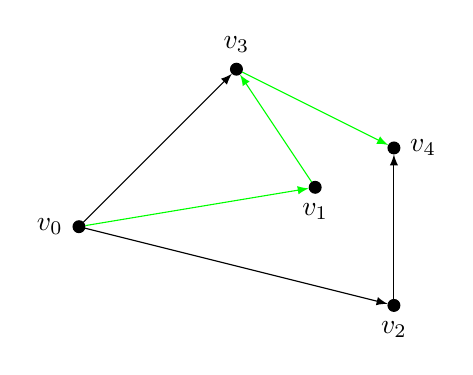
\begin{tikzpicture}

      \tikzset{enclosed/.style={draw, circle, inner sep=0pt, minimum size=.15cm, fill=black}}
%% Vertices
      	\node[enclosed, label={left: $v_0$}] (v0) at (0,2) {};
      	\node[enclosed, label={below: $v_1$}] (v1) at (3,2.5) {};
    		\node[enclosed, label={below: $v_2$}] (v2) at (4,1) {};
  	    \node[enclosed, label={above: $v_3$}] (v3) at (2,4) {};
     	\node[enclosed, label={right: $v_4$}] (v4) at (4,3) {};
%Edges
		\path [->, >=latex, green](v0) edge node[midway, sloped, above] {} (v1);
		\path [->, >=latex](v0) edge node[midway, sloped, above] {} (v2);
		\path [->, >=latex](v0) edge node[midway, above] {} (v3);
		\path [->, >=latex, green](v1) edge node[near end, sloped, below] {} (v3);
		\path [->, >=latex](v2) edge node[midway, below] {} (v4);
		\path [->, >=latex, green](v3) edge node[near end, sloped, above] {} (v4);

	\end{tikzpicture}
	\caption{Eksempel på en orienteret simpel graf og en vej fra $v_{0}$ til $v_{4}$}
	\label{fig.vaegtetopg}
\end{figure}


Antallet af veje mellem to knuder i grafen kan findes ved hjælp af nabomatricer, som vi diskuterede i forrige afsnit.
\begin{thm}
[Antallet af veje mellem to knuder] 
Lad G være en vilkårlig graf med nabomatricen
\textbf{$A$} med grafens knuder i rækkefølgen $v_{1},v_{2},\cdots,v_{n}$. Antallet af forskellige veje med længde $r$ fra $v_{i}$ til $v_{j}$ vil da være lig den $(i,j)$'te indgang af \textbf{$A^{r}$}.
\end{thm}

\begin{proof}
Bevis: Lad G være en graf med nabomatricen 
\textbf{$A$}, hvor vi antager, at knuderne i $G$ har rækkefølgen $v_{1},v_{2},\cdots,v_{n}$. Antallet af veje fra $v_{i}$ til $v_{j}$ af længde 1 er da den $(i,j)$'te indgang til 
\textbf{$A$}. Dette skyldes, at det blot er antallet af kanter fra $v_{i}$ til $v_{j}$.
Vi antager, at den $(i,j)$'te indgang til 
\textbf{${A^r}$} er antallet af forskellige veje, som går fra $v_{i}$ til $v_{j}$ og som har længden $r$. Dette er hypotesen, vi ønsker at bekræfte.
Vi ser på nabomatricen \textbf{$A^{r+1}$}. 
\textbf{$A^{r+1}$} er det samme som 
\textbf{$A^{r}$}$\cdot$\textbf{$A$}, og derfor er den $(i,j)$'te indgang af \textbf{$A^{r+1}$} lig med $b_{i1}a_{1j} + b_{i2}a_{2j} +\cdots+ b_{in}a_{nj}$. Her er $b_{ik}$  den $(i,k)$'te indgang til 
\textbf{$A^{r}$}, som ifølge vores hypotese er antallet af veje fra $v_{i}$ til $v_{k}$ med længde $r$.
En vej af længde $r + 1$ fra $v_{i}$ til $v_{k}$ er lavet ud fra en vej med længden $r$ fra begyndelsesknuden $v_{i}$ og hen til en mellemliggende knude $v_{k}$ samt den kant, der går fra $v_{k}$ til $v_{j}$. Vi ved fra kombinatorik, at antallet af muligheder er lig produktet af mulighederne ved første udfald og mulighederne ved andet udfald. Vi betegner antallet af veje med længden $r$ fra $v_{i}$ til $v_{k}$ med $b_{ik}$ og antallet af kanter fra $v_{k}$ til $v_{j}$ med $a_{kj}$ Finder vi produktet af dette for alle mellemliggende knuder, $v_{k}$, fås det ønskede resultat.
\end{proof}

\begin{exmp}
Vi starter med at kigge på en graf og den tilhørende nabomatrice:
\begin{figure}[H]
\centering
	\begin{tikzpicture}

      \tikzset{enclosed/.style={draw, circle, inner sep=0pt, minimum size=.15cm, fill=black}}
%% Vertices
      	\node[enclosed, label={left: $v_0$}] (v0) at (1,2) {};
      	\node[enclosed, label={above: $v_1$}] (v1) at (3,4) {};
    	\node[enclosed, label={below: $v_2$}] (v2) at (1,0) {};
  	    \node[enclosed, label={right: $v_3$}] (v3) at (5,2) {};
     	\node[enclosed, label={below: $v_4$}] (v4) at (5,0) {};
%Edges
		\path (v0) edge node[midway, sloped, above] {} (v1);
		\path (v0) edge node[midway, sloped, above] {} (v2);
		\path (v0) edge node[midway, above] {} (v3);
		\path (v1) edge node[near end, sloped, below] {} (v3);
		\path (v2) edge node[midway, below] {} (v4);
		\path (v3) edge node[near end, sloped, above] {} (v4);

	\end{tikzpicture}
	\caption{Eksempel på en ikke-orienteret simpel graf}
	\label{fig.vaegtetopg}
\end{figure}


\begin{equation}
A=\begin{bmatrix}
    0&1&1&1&0\\
    1&0&0&1&0\\
    1&0&0&0&1\\
    1&1&0&0&1\\
    0&0&1&1&0\\
\end{bmatrix}
\end{equation}


Vi ønsker at finde ud af hvor mange veje med en længde på 4, der går fra $v_0$ til $v_4$. Det ses i nabomatricen, at $v_0$ har 3 naboer, nemlig $v_1$, $v_2$ og $v_3$. Fortsætter vi, kan vi se, at $v_1$ har $v_0$ og $v_3$ som naboer, $v_2$ har $v_0$ og $v_4$, og $v_3$ har $v_0$, $v_1$ og $v_4$ som naboer. Fortsætter vi, så vi finder alle tænkelige veje med længder på 3, får vi, at der er 18 forskellige veje, der alle starter i $v_0$ og har en længde på 4. Vi skal nu finde de veje der ved at tilføje en kant ender i $v_4$. Vi kan se, at $v_4$ har $v_2$ og $v_3$ som naboer. Vi finder derfor de veje der starter i $v_0$ og slutter i $v_2$ med længden 3 og derefter dem der slutter i $v_3$ med længden 3. På denne måde udnytter vi, hvad vi skrev i beviset, nemlig at
\textbf{$A^{r+1}$} er lig med $b_{i1}a_{1j} + b_{i2}a_{2j} +\cdots+ b_{in}a_{nj}$
Her er $b_{ik}$ antallet af veje fra $v_{i}$ til ${v_k}$. I vores eksempel er $v_{i}=v_{0}$, ${v_k}=v_{2}$ og ${v_k}=v_{3}$ og \textbf{$A^{r+1}$}=\textbf{$A^{3+1}$}. 
 
\begin{figure}[H]
\centering
	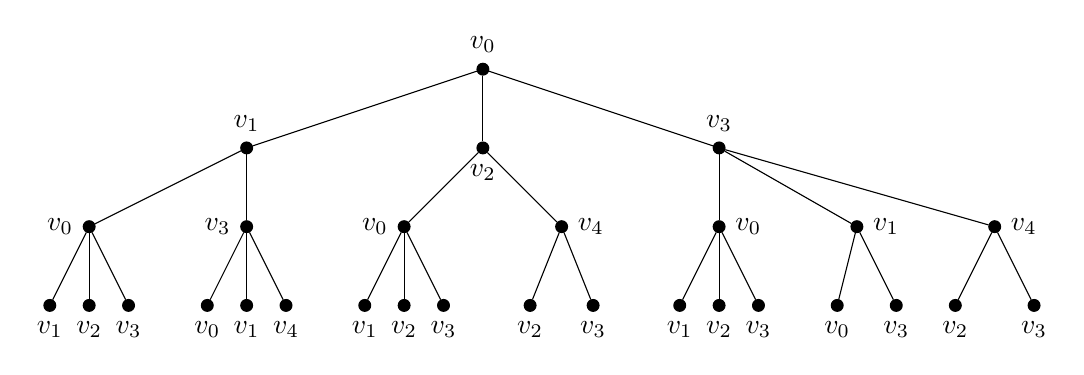
\begin{tikzpicture}

      \tikzset{enclosed/.style={draw, circle, inner sep=0pt, minimum size=.15cm, fill=black}}
%% Vertices
      	\node[enclosed, label={above: $v_0$}] (v0) at (3,6) {};
      	\node[enclosed, label={above: $v_1$}] (v1) at (0,5) {};
    		\node[enclosed, label={below: $v_2$}] (v2) at (3,5) {};
  	    \node[enclosed, label={above: $v_3$}] (v3) at (6,5) {};
     	\node[enclosed, label={left: $v_0$}] (v4) at (-2,4) {};
     	\node[enclosed, label={left: $v_3$}] (v5) at (0,4) {};
     	\node[enclosed, label={left: $v_0$}] (v6) at (2,4) {};
     	\node[enclosed, label={right: $v_4$}] (v7) at (4,4) {};
     	\node[enclosed, label={right: $v_0$}] (v8) at (6,4) {};
     	\node[enclosed, label={right: $v_1$}] (v9) at (7.75,4) {};
     	\node[enclosed, label={right: $v_4$}] (v10) at (9.5,4) {};
     	\node[enclosed, label={below: $v_1$}] (v11) at (-2.5,3) {};
      	\node[enclosed, label={below: $v_2$}] (v12) at (-2,3) {};
  	    \node[enclosed, label={below: $v_3$}] (v13) at (-1.5,3) {};
  	    \node[enclosed, label={below: $v_0$}] (v14) at (-0.5,3) {};
     	\node[enclosed, label={below: $v_1$}] (v15) at (0,3) {};
     	\node[enclosed, label={below: $v_4$}] (v16) at (0.5,3) {};
     	\node[enclosed, label={below: $v_1$}] (v17) at (1.5,3) {};
      	\node[enclosed, label={below: $v_2$}] (v18) at (2,3) {};
  	    \node[enclosed, label={below: $v_3$}] (v19) at (2.5,3) {};
  	    \node[enclosed, label={below: $v_2$}] (v20) at (3.6,3) {};
  	    \node[enclosed, label={below: $v_3$}] (v21) at (4.4,3) {};
  	    \node[enclosed, label={below: $v_1$}] (v22) at (5.5,3) {};
      	\node[enclosed, label={below: $v_2$}] (v23) at (6,3) {};
  	    \node[enclosed, label={below: $v_3$}] (v24) at (6.5,3) {};
  	    \node[enclosed, label={below: $v_0$}] (v25) at (7.5,3) {};
     	\node[enclosed, label={below: $v_3$}] (v26) at (8.25,3) {};
     	\node[enclosed, label={below: $v_2$}] (v27) at (9,3) {};
     	\node[enclosed, label={below: $v_3$}] (v28) at (10,3) {};
%Edges
		\path (v0) edge node[midway, sloped, above] {} (v1);
		\path (v0) edge node[midway, sloped, above] {} (v2);
		\path (v0) edge node[midway, above] {} (v3);
		\path (v1) edge node[near end, sloped, below] {} (v4);
		\path (v1) edge node[midway, below] {} (v5);
		\path (v2) edge node[near end, sloped, above] {} (v6);
		\path (v2) edge node[near end, sloped, above] {} (v7);
		\path (v3) edge node[near end, sloped, above] {} (v8);
		\path (v3) edge node[near end, sloped, above] {} (v9);
		\path (v3) edge node[near end, sloped, above] {} (v10);
		\path (v4) edge node[near end, sloped, above] {} (v11);
		\path (v4) edge node[near end, sloped, above] {} (v12);
		\path (v4) edge node[near end, sloped, above] {} (v13);
		\path (v5) edge node[near end, sloped, above] {} (v14);
		\path (v5) edge node[near end, sloped, above] {} (v15);
		\path (v5) edge node[near end, sloped, above] {} (v16);
		\path (v6) edge node[near end, sloped, above] {} (v17);
		\path (v6) edge node[near end, sloped, above] {} (v18);
		\path (v6) edge node[near end, sloped, above] {} (v19);
		\path (v7) edge node[near end, sloped, above] {} (v20);
		\path (v7) edge node[near end, sloped, above] {} (v21);
		\path (v8) edge node[near end, sloped, above] {} (v22);
		\path (v8) edge node[near end, sloped, above] {} (v23);
		\path (v8) edge node[near end, sloped, above] {} (v24);
		\path (v9) edge node[near end, sloped, above] {} (v25);
		\path (v9) edge node[near end, sloped, above] {} (v26);
		\path (v10) edge node[near end, sloped, above] {} (v27);
		\path (v10) edge node[near end, sloped, above] {} (v28);

	\end{tikzpicture}
	\caption{De mulige løsninger for veje med længde 3 fra $v_{0}$ til $v_{k}$}
	\label{fig.vaegtetopg}
\end{figure}

Antallet af veje fra $v_{0}$ til $v_{2}$ er 5 og antallet af veje fra $v_{0}$ til $v_{3}$ er 6. Vi kan derfor opstille
\textbf{$A^{4}$}$=b_{1i} \cdot a_{1j}+b_{2i} \cdot a_{2j}=5 \cdot 1+6 \cdot 1=11$
Her er $b_{1i}$ antallet af veje fra $v_{i}=v_{0}$ til vores første $v_{k}=v_{2}$ og $a_{1j}$ er antallet af kanter fra vores første $v_{k}=v_{2}$ til vores $v_{j}=v_{4}$. På samme måde optræder $b_{2i}$ og $a_{2j}$ for vores andet $v_{k}=v_{3}$. Der er altså 11 veje med længden 4 fra knuden $v_{0}$ til knuden $v_{4}$.

\end{exmp}

\subsection{Vægtede grafer}
En \emph{vægtet graf} er en graf, hvori kanterne eller knuderne får tildelt en numerisk værdi. I dette projekt arbejdes der udelukkende med vægtede kanter, og vi vil derfor kun fokusere på dem i dette afsnit.
En vægtet graf er defineret ved:
\begin{defn}[Vægtede grafer]
En vægtet graf, $G=(V,E,w)$, består af en mængde knuder, $V$, en mængde kanter, $E$, og \emph{vægtfunktionen}, $w: E \rightarrow \R$.
\end{defn}

For en vægtet graf har alle kanter $e\in E$ en numerisk vægt, givet ved funktionen $w (e)$. Da $e$ er en kant incident med $\{u,v\}$ kan man ligeledes skrive $w (u,v)$. På samme måde som med uvægtede grafer, kan en vægtet graf også opdeles i de seks graftyper fundet i tabel \ref{tab:typer}.
\input{fig/tikz/grafer/veje/vægtede/eksempel}

Da vægtede grafer har en numerisk vægt på hver kant, kan man således beregne \emph{distancen} fra en knude til en anden i grafen. Distancen fra en knude til en anden kan defineres således:

\begin{defn}[Distance]
Lad $m\in \N $, $G=(V,E,w)$ være en vilkårlig graf og  $e_{v_i,v_{i+1}}$ være en kant, som er incident med $v_i$ og $v_{i+1}$. Lad en tilfældig, simpel vej, $P$, gå igennem knuderne således $P=(v_{1},v_{2},\dotsc,v_{m})$, da kan distancen beskrives som
	\begin{equation*}
	\mathrm{dist}(P)=\sum_{i=1}^{m}w(e_{v_i,v_{i+1}}).
	\end{equation*}  
\end{defn}

Man kan således bruge følgende definitioner af \emph{korteste vej} og \emph{længste vej} i en vægtet graf:


\begin{defn} [Korteste vej i vægtet graf]\label{defn:min.vej}
Lad $G=(V,E,w)$ være en vilkårlig, vægtet graf. Da er distancen af den korteste vej, fra en knude, $v_1$, til en anden knude, $v_m$, defineret som
	\begin{equation*}
		\alpha(v_1,v_m)=\arg \min_{P \in \euscr{P}}
		\textrm{dist}(P),
	\end{equation*}
	hvor $\euscr{P}$ er mængden af alle veje fra $v_1$ til $v_m$.
\end{defn}

På samme vis defineres længste vej:

\begin{defn} [Længste vej i en vægtet graf]
	Lad $G=(V,E,w)$ være en vilkårlig, vægtet graf. Da er distancen af den længste vej, fra en knude, $v_1$, til en anden knude, $v_m$, defineret som
	\begin{equation*}
		\beta(v_1,v_m)=\arg \max_{P \in \euscr{P}}
		\textrm{dist}(P),
	\end{equation*}
	hvor $\euscr{P}$ er mængden af alle veje fra $v_1$ til $v_m$.
\end{defn}

\begin{exmp}
Betragt figur \ref{fig.vaegtetopg} \\
\input{fig/tikz/grafer/veje/vægtede/opgave}
På figuren ses en graf med vægtede kanter. Vi er interesserede i at finde den korteste vej fra $v_1$ til $v_6$. For at finde den korteste vej, kigger vi på alle de mulige veje fra $v_1$ til $v_6$.
Følgende veje ses:
\begin{align*}
	P_1=&(v_1,v_2,v_4,v_6)\\
	P_2=&(v_1,v_2,v_5,v_6)\\
	P_3=&(v_1,v_3,v_5,v_6)\\
	P_4=&(v_1,v_3,v_4,v_6)
\end{align*}
Man kan nu beregne distancen af de fire veje, ved at tage summen af de kanter, vejen følger. Man får derved:
\begin{align*}
	P_1=&4+3+2=9\\
	P_2=&4+6+1=11\\
	P_3=&5+3+1=9\\
	P_4=&5+1+2=8
\end{align*}
Det ses, at den korteste vej fra $v_1$ til $v_6$ er $P_4$. 
Det er sådan, man kan finde korteste vej i en vægtet graf. Denne metode kaldes \emph{brute force}. Metoden kan blive meget tidskrævende ved mere komplekse grafer. I disse tilfælde vil man bruge alternative, bedre algoritmer til at løse problemet. Dette vil vi komme ind på senere i kapitel \ref{kap.algo}.
\end{exmp}


\section{Delte grafer}
I visse tilfælde kan en graf deles op for at optimere en algoritme til løsningen af en given problemstilling.
To mulige grafopdelinger er delgrafer og $k$-delte grafer.

\begin{defn}[Delgraf] \label{defn:delgraf} %subgraph
En \emph{delgraf} af grafen, $G= (V,E)$, er en graf, $D = (W,F)$, skabt af delmængderne af kanterne, $F \subseteq E$, og knuderne, $W \subseteq V$, hvori det gælder $F \subseteq (\{u,v\} | u,v \in W)$.
\end{defn}

En delgraf er \emph{induceret}, hvis mængden af kanter, $F$, indeholder alle kanter fra $E$, hvis knuder indgår i $W$.
Delgrafen kaldes \emph{udspændende} hvis $W=V$. 

\begin{defn}[\emph{k}-delt] \label{defn:k-delt} %k-partite
En graf, $G = (V, E)$, kaldes en \emph{$k$-delt graf}, hvis $V$ kan deles op i $k$ ikke-tomme delmængder, $V_1, V_2,\dotsc, V_k$, således at $V= V_1 \bigcup V_2 \bigcup \dotsc \bigcup V_k$. Foruden gælder det at $V_i \bigcap V_j  = \emptyset \forall i,j$, og $i\neq j$. Samtidigt kan to vilkårlige knuder, $v$ og $u$, kun være naboer, hvis de befinder sig i forskellige delmængder. 
\end{defn}

Vi ved fra \autoref{kap:vaegtede}, at den optimale delstruktur findes, når man løser et korteste vej-problem. Dermed findes den optimale delstruktur, $D_{ij}$, hvis den optimale delgraf, $D$, er fundet.










\include{incl/main/formalia/analyse}
\chapter{Vurdering af metoderne}
\section{Sektion 1}

\section{Sektion 2}

\section{Sektion 3}
\chapter{Konklusion}

\subsection{Økonomi}

Vi kan jo få lidt økonomi ind over det? 

Normalt set vil man altid gøre denne slags investeringer, hvis det giver overskud, men da der ikke er taget højde for omkostninger som løn, maskiner og andet, er det svært at konkludere om det vil give mening at gennemføre denne investering.?
Skal vi skrive noget i stil med det?
%\chapter{Forord}
Følgende projekt er udarbejdet af gruppe B350 bestående af fem stud.scient.oeconer på 1. semester. Projektet er skrevet i efteråret 2020 og beskæftiger sig med diskret matematik herunder optimering af et gaslager som basisproblem. Diskret matematik indgår i studiets læreplan og er derfor et relevant emne til projektskrivning. Projektet er skrevet i \LaTeX, og delt via GitAhead.
Vi vil som gruppe rette en stor tak til vores vejleder Janus Valberg-Madsen for godt samarbejde gennem projektforløbet samt gode råd og rettelser.






% Input-filer bør opdeles således, at hver fil svarer til et kapitel. Makroen
% \include indsætter et sideskift og indholdet fra den givne stil.

% \include{incl/main/example1}
% \include{incl/main/example2}
% ...

% Appendicer indsættes inde i en appendices-blok og bliver nummereret med
% bogstaver i stedet for tal
\begin{appendices}
  % \include{incl/app/appendix1}
  % \include{incl/app/appendix2}
  % ..
\end{appendices}

% Dokumentets 'back matter' er til ekstra ting som f.eks. litteraturlisten.
% Overskrifter bliver ikke nummereret her.
\backmatter

% Automatisk litteraturliste baseret på, hvilke kilder, der er blevet refereret
% til i løbet af rapporten.
\bibliographystyle{apalike}
\bibliography{
  incl/bib/books,
  incl/bib/articles,
  incl/bib/software
}
\end{document}
